%%% Document formatting %%%
\documentclass[
    a4paper, 
    stu,
    biblatex,
    %draftfirst,
    helv,
    floatsintext,
    11pt,
]{apa7}

\title{The Challenges and Rewards of Analysing Handwritten Records}
\authorsnames{Antriksh Dhand}
\authorsaffiliations{{School of Medical Sciences, The University of Sydney}}

\course{SCDL3991: Science Dalyell Individual Research Project}
\duedate{15th June, 2024}
\professor{Dr. Rebekah A. Jenkin and Professor Kevin Keay}

\abstract{This research project investigates the challenges and rewards of analysing historical handwritten records through an analysis of Anatomy Registers at The University of Sydney. This paper discusses data verification, validation, and transformation techniques applied to improve data quality and prepare the dataset for meaningful analysis. It highlights the methods used for data standardisation and categorisation, and provide insights into societal trends over time through a geographical analysis of the data.}

\addbibresource{bibliography.bib}

%%% Image packages %%%
\usepackage{graphicx}
\graphicspath{ {./img/} }

%%% Tables %%%
\usepackage{booktabs}
\usepackage{multirow}
\usepackage{pdflscape} % Rotate tables

%%% Text %%%
\usepackage{hyperref} % hyperlinks
\hypersetup{
hidelinks,
colorlinks=false,
pdftitle={SCDL3991 Final Report},
pdfpagemode=FullScreen
}
\usepackage{setspace} % line spacing
\usepackage{lipsum} % lorem ipsum paragraphs
\usepackage{nameref} % named references to sections for APA

%%% CODE INPUT %%%
\usepackage{listings}
\definecolor{backcolour}{rgb}{0.95,0.95,0.92}
\definecolor{codegray}{rgb}{0.5,0.5,0.5}
\definecolor{backgray}{RGB}{235, 235, 235}

% Code input styling
\lstset{
    language=Python,
    basicstyle=\linespread{1.2}\ttfamily\small,
    numbers=left,
    numberstyle=\tiny\color{codegray},
    columns=fixed,
    breaklines=true,
    backgroundcolor=\color{backcolour},
    frame=single,
    showstringspaces=false,
    commentstyle=\color{codegray},
    literate={~} {$\sim$}{1},
    upquote=true
}

% Code output styling
\lstdefinestyle{output}{
    basicstyle=\linespread{1.2}\ttfamily\small,
    backgroundcolor=,
    numbers=none,
    frame=single,
    breaklines=true,
}

\begin{document}

% TITLE PAGE %
%------------------------------------------------------------------%

\maketitle

%------------------------------------------------------------------%

The intersection of computational techniques with humanities research has historically encountered both skepticism and gradual acceptance \parencite{macroanalysis_digital_humanities, big_data_history}. As early as the 1980s, the legitimacy of computer-based work in humanities was under debate, often seen as too ``mechanical'' for the exploration of human culture and history \parencite{olsen_1993, hockey_2004}. It wasn't until the turn of the century when advanced processing capabilities, simpler programming interfaces, and greater data availability came into fruition that the potential of ``digital humanities'' as a field of academia began to be recognised more broadly \parencite{dh_history}.

This project is uniquely positioned at such an intersection, specifically intertwining humanities, anatomy, and data science. The broad aim of our project is to attain a better understanding of changes in anatomy body procurement practices during the formation of modern Australia. Central to this are the Anatomy Registers from The University of Sydney School of Medical Science, which chronicle over a century of body acquisition for anatomical study. This extensive dataset not only shows the evolution of medical and scientific practices in the nineteenth and twentieth centuries, but also opens a window to the sociocultural and ethical dimensions of the era. By exploring these registers, we are exploring how societal values, medical ethics, and the law all interact with the scientific pursuit of knowledge.

\subsection{Background}

In the digital era, it might seem that all necessary data for addressing contemporary challenges is readily available in a structured, digital format. In reality, researchers are repeatedly falling back onto the troves of information locked away in historical records to make ground on their inquiries -- information which often remains underutilised due to its non-digital or unstructured format \parencite{big_data_history}.

\paragraph{Sea level records}{One domain which has found good use of digitising archival records is the domain of geological sciences, specifically, the field of oceanography. A rise in global sea levels is expected to be one of the most devastating and costly effects of climate change in the next century \parencite{mimura_2013_sea}, and thus, having accurate data on sea levels across the world is essential for scientists to correctly understand the mechanisms involved behind these trends \parencite{marcos_2011_cadiz}. However, historical sea level data -- crucial for long-term analyses -- often only exists in analogue form, as digital recording only became prominent in the late 20th century. Consequently, current datasets might be inadequate for centennial-scale forecasting \parencite{talke_2020_columbia_river}. Recognising this gap, extensive digitisation efforts have emerged globally, including in Spain \parencite{marcos_2011_cadiz, marcos_2013_tenerife, marcos_2021_spain}, North America \parencite{talke_2014_new_york, talke_2018_boston, talke_2020_columbia_river}, France \parencite{woppelmann_2014_marseille}, and the United Kingdom \parencite{inayatillah_2022_thames}. These projects have significantly contributed to databases such as \textit{Système d'Observation du Niveau des Eaux Littorales} (\href{https://www.sonel.org/?lang=en}{SONEL}), which support ongoing oceanographic research \parencite{lyszkowicz_2019_baltic}.}

\paragraph{Ship logbooks}{Researchers including Kostas Petrakis have aimed to uncover truths about the transition from sail to steam navigation in the Mediterranean through digitising and analysing ship logbooks from the nineteenth and twentieth centuries. Despite the challenges posed by outdated navigational references and archaic language unfamiliar to contemporary scholars, the records have helped trace out the expansion of maritime routes due to the advent of steam ships, and also the psychological impact on those experiencing these shifts firsthand: \textit{``In the margin of the logbook [the captain] wrote twice about his disappointment and frustration...`The screw broke and I don’t know what to do, one difficulty after the other. God help me because I am going to lose my mind!'''} \parencite{petrakis_2021_ship}. It would be rare for such emotional insights to be captured through traditional research involving shipping records or calendars.}

The above examples highlight the value of the research described in this project: transcribing and analysing historical data helps researchers attain a greater understanding of the physical and sociocultural changes occurring throughout history.

\subsection{Project Scope}

Originally the project aspirations were quite broad. For example, one of the initial aims of the project was to map advances in medical knowledge and diagnosis granularity through analysing changes in cause of death terminology. This was to be conducted through a technique called ``dynamic topic modelling'' \parencite{blei_2006_dtm}, which utilises unsupervised machine learning techniques to extract the $n$ most prevalent topics from a corpus of text. However, the limitations of using hand-transcribed records soon became apparent. For example:

\begin{enumerate}
    \item No formal data cleaning procedure had been conducted on the dataset;
    \item Historical records are usually transcribed with the aim of extracting an accurate account of events or people and not necessarily for the purposes of analysis. Due to this, no \textit{deliberate} alterations were made from the source material during transcription e.g. fixing misspellings;
    \item The process of digitising records written in traditional cursive scripts is incredibly laborious and error-prone.
\end{enumerate}

Furthermore, though analysis on the dataset had been conducted before, none focused on geographical location or cause of death and as such these attributes were still in their raw form. The project aim thus shifted to (1) using programming techniques to transform the transcriptions into useable data; and (2) completing a geographical mapping of the place of death of all bodies received.
\newpage
\section{Methodology}

This section will describe the methods used to improve the data quality of the Anatomy Registers dataset. All analysis work done was conducted using the Python programming language, specifically, the data processing library \texttt{pandas}. The appendices contain the complete analysis files.

\subsection{Introduction to the dataset}

The Anatomy Registers of The University of Sydney Medical School are a significant data repository that record the sourcing of human bodies for anatomical study from 1883 to present. Detailed records pertaining to the 7609 bodies received between 1883 to 1983 were transcribed into a digital dataset \parencite{rebekah_jenkin} and were deidentified for use in this project in accordance with ethics (approval number 2017/898).

The data, when contextualised with historical events, legal changes, and shifts in medical practices, allows for a comprehensive understanding of how societal values and norms influenced medical science. For example, in part due to a ``lack of public awareness of the value and importance of donating bodies for dissection'' \parencite{rebekah_jenkin}, there was an extreme shortage of bodies for anatomical dissection during the 1940s and 1950s (Figure \ref{fig:ida-by-year}). Additionally, the dataset reveals a predominant male to female ratio, reflecting the gender disparities in residents of the asylums of the time (Figure \ref{fig:ida-by-sex}). 

\begin{figure}[p]
    \centering
    \caption{Number of entries in USYD Anatomy Registers by year}
    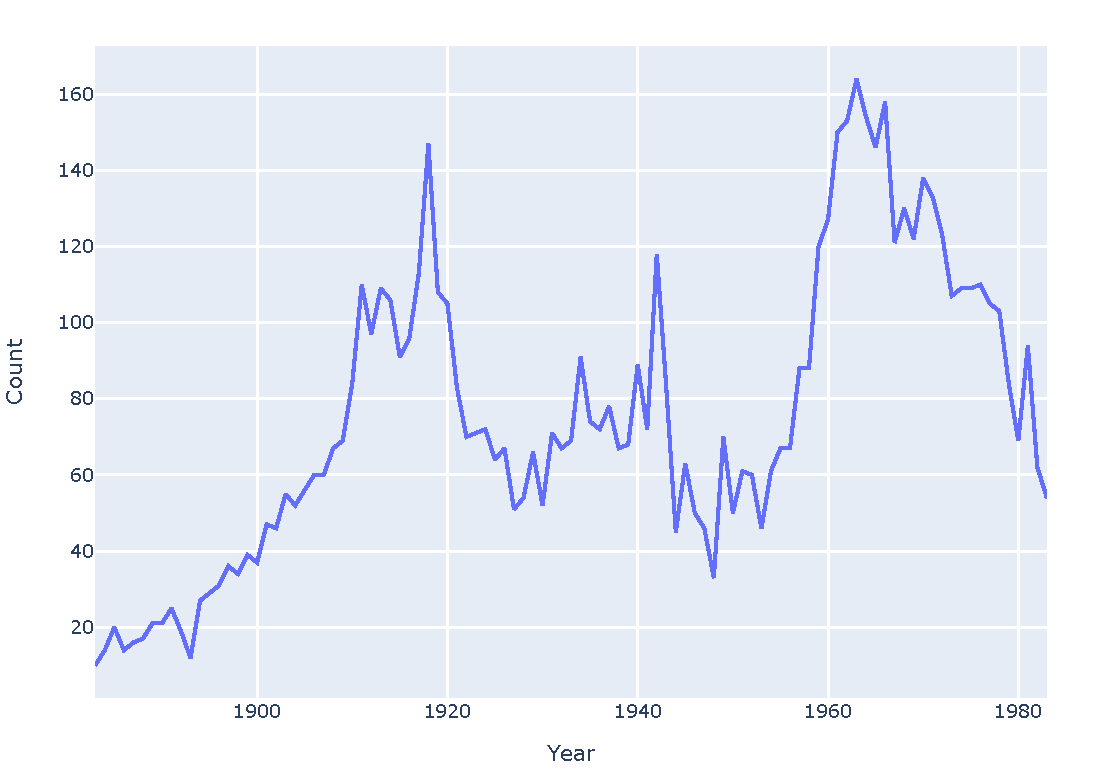
\includegraphics[width=0.9\textwidth]{REPORT/img/data_by_year.pdf}
    \label{fig:ida-by-year}
\end{figure}

\begin{figure}[p]
    \centering
    \caption{Sex of bodies received over time}
    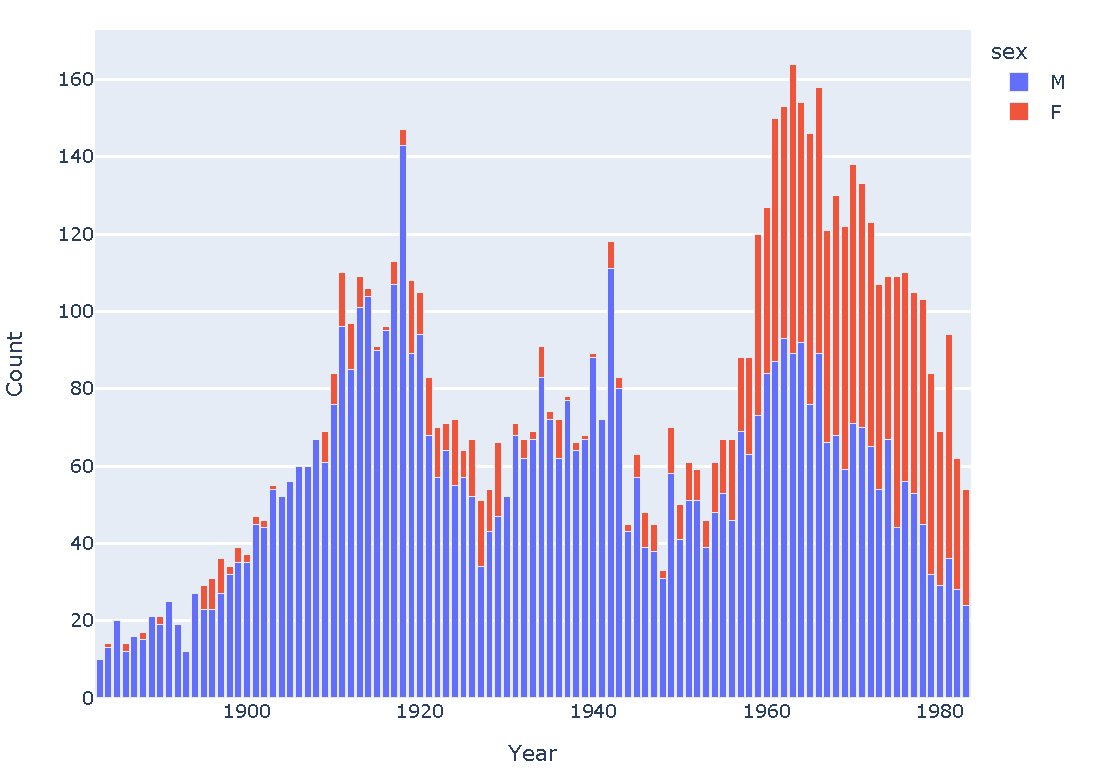
\includegraphics[width=0.9\textwidth]{REPORT/img/data_by_sex.pdf}
    \label{fig:ida-by-sex}
\end{figure}

\subsection{Data verification and validation}\label{subsec:data-v-v}

Data quality can broadly be determined through three factors: (a) data completeness; (b) data consistency; and (c) data validity. 

%%%%%%%%%%%%%%%%%%%%%%%%%%%%%%%
\subsubsection{Data completeness}
%%%%%%%%%%%%%%%%%%%%%%%%%%%%%%%

Data completeness refers to the extent that all expected records and attributes are present in a dataset. Initially, several of our attributes contained missing values (see Table \ref{tab:missing-values}). 


\paragraph{Imputing missing values} Over 2403 entries in the dataset were missing a date of death. However, there were zero missing entries for the date of reception. The date of reception was usually on, or close to (two to three days after) the patient's death. Therefore, the date of reception values were used to impute the missing values of the date of death attribute.

\begin{table}[p]
\centering
\caption{Missing values for attributes in the Anatomy Registers dataset before and after data cleaning}
\label{tab:missing-values}
\singlespacing
\begin{tabular}{@{}lrr@{}}
\toprule
\textbf{Attribute}                        & \textbf{NULL entries before cleaning} & \textbf{NULL entries after cleaning} \\ \midrule
year                    & 0                               &  0                             \\
id                      & 0                               &  0                             \\
sex                     & 5                               &  0                             \\
age                     & 10                              &  0                             \\
death\_date             & 2436                            &  0                             \\
reception\_date         & 0                               &  0                             \\
return\_date\_sepulture & 1680                            &  1673                          \\
burial\_date            & 4408                            &  4394                          \\
death\_place            & 6                               &  0                             \\
place\_code             & 0                               &  0                             \\ \bottomrule
\end{tabular}
\end{table}

\paragraph{Removing entries with missing values} 15 cases had missing values for age, sex or place of death.  As these characteristics could not be imputed from other information, these entries were removed from the dataset. 

%%%%%%%%%%%%%%%%%%%%%%%%%%%%%%%
\subsubsection{Data consistency}
%%%%%%%%%%%%%%%%%%%%%%%%%%%%%%%

Data consistency refers to the dataset adhering to a set of rules and formats. More practically, it involves ensuring each attribute in a dataset fits the most precise datatype it can.

\paragraph{Checking dates}{A regular expression (regex) was utilised to check if dates were in the standard DD/MM/YYYY format.
\begin{equation}
    \texttt{\textasciicircum(0?[0-9]|[12]\textbackslash d|3[01])\/(0?[0-9]|1[0-2])\/(000\textbackslash d|00\textbackslash d\{2\}|0\textbackslash d\{3\}|1\textbackslash d\{3\}|2000)\$}
\end{equation}

Some of the erroneous entries discovered through this method can be seen in Table \ref{tab:error-dates}. In total there were 21 such entries, ranging from a missing forward slash (``/'') in the date to the word ``missing'' or ``[blank]'' being used to indicate a missing value. These entries were then individually corrected by hand.}

\begin{table}[htbp]
\centering
\caption{A few erroneous date entries from each date column}
\label{tab:error-dates}
\begin{tabular}{@{}cllll@{}}
\toprule
\textbf{id} & \textbf{death\_date} & \textbf{reception\_date} & \textbf{return\_date\_sepulture} & \textbf{burial\_date} \\
\midrule
1898 & 25/1/2020 & \ldots & \ldots & \ldots \\
5014 & 26/87/1961 & \ldots & \ldots & \ldots \\
5044 & 20/11/9161 & \ldots & \ldots & \ldots \\
7116 & 5/101977 & \ldots & \ldots & \ldots \\
1727 & \ldots & missing & \ldots & \ldots \\
2408 & \ldots & 23 /4/1925 & \ldots & \ldots \\
2644 & \ldots & \ldots & crossed out 27/9/1929 & \ldots \\
3184 & \ldots & \ldots & [blank] & \ldots \\
3185 & \ldots & \ldots & [blank] & \ldots \\
3203 & \ldots & \ldots & [blank] & \ldots \\
6726 & \ldots & \ldots & \ldots & 04/04//1975 \\
\bottomrule
\end{tabular}
\end{table}


%%%%%%%%%%%%%%%%%%%%%%%%%%%%%%%
\subsubsection{Data validity}
%%%%%%%%%%%%%%%%%%%%%%%%%%%%%%%

Data validity refers to the data accurately representing the real-world values it is supposed to depict -- i.e. the values in the dataset should make sense. Some of the checks conducted are listed below:
\begin{itemize}
    \item Checking the range of \texttt{death\_date} and \texttt{reception\_date} (should be between 1883 and 1983)
    \item Checking that \texttt{death\_date} and \texttt{reception\_date} were no longer than 10 days apart
    \item Checking that \texttt{death\_date} is always less than or equal to \texttt{reception\_date}
\end{itemize}

56 invalid entries were found due to the above checks, mostly due to typos when entering dates. Most of these were corrected by double-checking with the original sources; a few were inferred through looking at surrounding entries for the correct values for day, month, or year.

\subsection{Data transformation}

It is difficult to apply traditional verification techniques such as those discussed in the previous section to the cause of death and place of death columns:

\begin{enumerate}
\item Cause of death and place of death are unstructured text attributes (unlike year, age, and dates).
\item Legislation mandated the maintenance of cause of death and place of death records but did not specify the level of detail required (see the Anatomy Acts of 1881, 1901, and 1977).
\item Medical advancements over the 20th century led to increasingly precise causes of death, with later entries often including detailed tertiary diagnoses.
\end{enumerate}

These attributes are therefore difficult to validate or analyse in their raw form. Hence, \textit{data transformation} was used in order to make programmatic analysis more feasible. Transforming the place of death attribute was our focus for this semester-long project.

%%%%%%%%%%%%%%%%%%%%%%%%%%%%%%%
\subsubsection{Categorising place of death}
%%%%%%%%%%%%%%%%%%%%%%%%%%%%%%%

Regular expressions and keyword analysis techniques were used to extract $\sim$7000 entries into 9 categories based on their place of death (see Table \ref{tab:categories}). For example, the following set of rules were developed to extract private residences:

\begin{table}
    \centering
    \caption{Categories extracted from the place of death attribute in the Anatomy Registers}
    \label{tab:categories}
    \begin{tabular}{ll}
        \toprule
        \textbf{Category} & \textbf{Classification criteria} \\
        \midrule
        Private residence & A private address (commencing with a street, flat, or unit number) \\
        Aged care & Locations containing ``Nursing'', ``Convalescent'', ``Aged Care'', \ldots \\
        Hospice & Locations containing ``Hospice'' + some known hospices \\
        Private hospital & Locations containing ``Private Hospital'' or ``surgery'' \\
        Public hospital & All hospitals without ``private'' in their name\\
        Public asylum & Macquarie St, Liverpool, George St, Rockwood \\
        Public mental asylum & Newingtown + locations containing ``mental asylum'' or ``psychiatric'' \\
        Aged 2 and under & Currently coded 70 \\
        Morgues & Locations containing ``morgue'' \\
        Other & Other \\
        \bottomrule
    \end{tabular}
\end{table}

\begin{enumerate}
    \item The location starts with ``flat'', ``unit'', ``lot'', or contains ``at home'' e.g. ``Flat 73, Darley St, Darlinghurst''
    \item The location starts with a digit, and also contains an address suffix e.g. ``5 York Rd, Bondi Junction''
\end{enumerate}

These rules were converted into regular expressions, and any entries which matched the expressions were categorised as ``private residence.'' A similar procedure was then repeated for each other category, such as ``private hospital'' or ``aged care''.

%%%%%%%%%%%%%%%%%%%%%%%%%%%%%%%
\subsubsection{Extracting suburbs from place of death}
%%%%%%%%%%%%%%%%%%%%%%%%%%%%%%%

In order to pursue a geographical analysis of the Anatomy Registers dataset, it was important to extract some form of location data from the place of death attribute. The most straightforward approach was to extract the suburb name, as it commonly appeared in the unstructured entries of both private residences and other categories of institutions.

A secondary dataset was first sourced which contained the names and geographical boundaries of all 4615 localities in NSW (see Tables \ref{tab:suburb-dataset-details} and \ref{tab:suburb-dataset-head}). Any suburb name present in each place of death entry was then extracted from the records using regular expressions.

\begin{table}[htbp]
\centering
\caption{Attribution details of the NSW Localities dataset}
\label{tab:suburb-dataset-details}
\begin{tabular}{@{}ll@{}}
\toprule
\textbf{Attribute}         & \textbf{Details} \\
\midrule
Dataset name               & NSW Local Government Areas - Geoscape Administrative Boundaries \\
Source                     & Data originally found on data.gov.au. Link here: \url{https://shorturl.at/DMbhb}\\
Attribution                & Licensed by the Commonwealth of Australia under Creative Commons \\
                           & Attribution 4.0 International licence (CC BY 4.0). \\
Last updated               & 27/02/2024 \\
\bottomrule
\end{tabular}
\end{table}

\begin{table}[htbp]
\centering
\caption{First few rows of the NSW Localities dataset}
\label{tab:suburb-dataset-head}
\begin{tabular}{@{}ll@{}}
\toprule
\textbf{suburb}      & \textbf{geometry}      \\ \midrule
Aarons Pass & \texttt{POLYGON (...)} \\
Abbotsbury  & \texttt{POLYGON (...)} \\
Abbotsford  & \texttt{POLYGON (...)} \\
Abercrombie & \texttt{POLYGON (...)} \\ 
Abercrombie River & \texttt{POLYGON (...)} \\
\ldots & \ldots \\ \bottomrule
\end{tabular}
\end{table}

Interestingly, 950 entries from the dataset contained more than one suburb; examples of these can be seen in Table \ref{tab:extract-all-suburbs}. This was mostly for the following reasons:
\begin{enumerate}
    \item An institution contains a suburb in its name but is physically addressed in a different suburb e.g. ``Berrima District Hopsital, Bowral'';
    \item A street shares its name with a suburb e.g. ``Clovelly Rd'';
    \item A combination of the above, often leading to three extracted suburbs e.g. ``Ryde Hospital, Denistone Rd, Eastwood''.
\end{enumerate}

\begin{table}[htbp]
\centering
\caption{A select few examples of place of death entries containing multiple suburbs}
\label{tab:extract-all-suburbs}
\resizebox{\textwidth}{!}{%
    \begin{tabular}{@{}lllll@{}}
    \toprule
    \textbf{id} & \textbf{death\_place} & \textbf{suburb\_1} & \textbf{suburb\_2} & \textbf{suburb\_3} \\ \midrule
    5122 & Corner Clovelly Rd \& Glebe Rd Randwick & Clovelly & Glebe & Randwick \\
    5533 & Berrima District Hospital, Bowral & Berrima & Bowral & - \\
    7567 & Ryde Hospital, Denistone Rd, Eastwood & Ryde & Denistone & Eastwood \\
    7596 & St George Nursing Home, 3 Verdun St, Bexley & St George & Bexley & - \\
    7598 & Kilbride Nursing Home, Appin Rd, Campbelltown & Appin & Campbelltown & - \\ \bottomrule
    \end{tabular}
}
\end{table}

These entries were cleaned programmatically by (a) checking if all classifications of an entry were identical and selecting any one of these classifications, and (b) if the place of death was an address, selecting the suburb which was extracted from the record \textit{last}, as the suburb always comes after the street name and institution name in an address. These steps correctly assigned over 800 of the 950 multiply assigned entries in the dataset.

The remaining entries which could not be condensed through the above procedure were entries with typos, such as ``2 balmoral \textit{avemue} croydon park''; conjunct entries, such as ``hornsby hospital \textit{from} oatlands nursing home dundas''; or institutions which had multiple suburbs in their names, such as ``\textit{ryde} district soldiers memorial hospital \textit{eastwood}''. These last entries were classified manually using a data entry UI created using Jupyter Notebook widgets (see Figure \ref{fig:data-entry-ui}).

\begin{figure}
    \centering
    \caption{Data entry UI made to classify entries manually}
    \label{fig:data-entry-ui}
    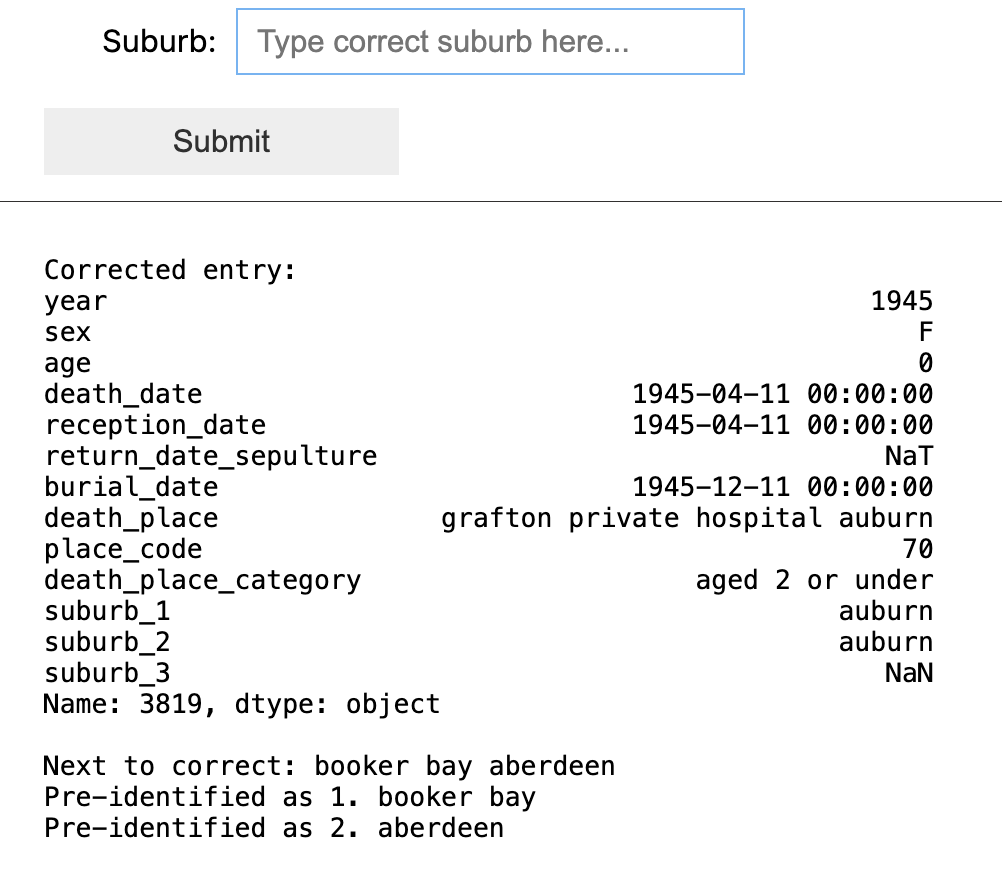
\includegraphics[width=0.6\textwidth]{REPORT/img/data_entry_ui.png}
\end{figure}

Finally, there were 478 entries in the dataset that did not contain any suburbs at all. A majority of these were hospital names, such as ``callan park mental hospital'' or ``dalcross private hospital'', and many contained misspelled suburbs which were unable to be picked up through the regex checker, such as ``wallandra private hospital \textit{marrickvillle}'' or ``outside 1018 francis avenue \textit{brightonlesands}''. These were also manually classified using a modified version of the data entry UI from Figure \ref{fig:data-entry-ui}.

After this process, there were only 86 entries in the dataset (1.33\%) which did not receive a suburb classification. As seen in Figure \ref{fig:missing-suburbs}, about two-thirds of the remaining entries can be attributed to deaths at unspecified morgues, and a large majority of the remaining one-third entries were neonatal deaths which did not routinely include a place of death in the record associated with their receipt by the Medical School. These 86 entries were subsequently dropped from the dataset in order to facilitate an accurate merge with the geographical dataset.

\begin{figure}
    \centering
    \caption{Categories of entries with missing suburb classifications}
    \label{fig:missing-suburbs}
    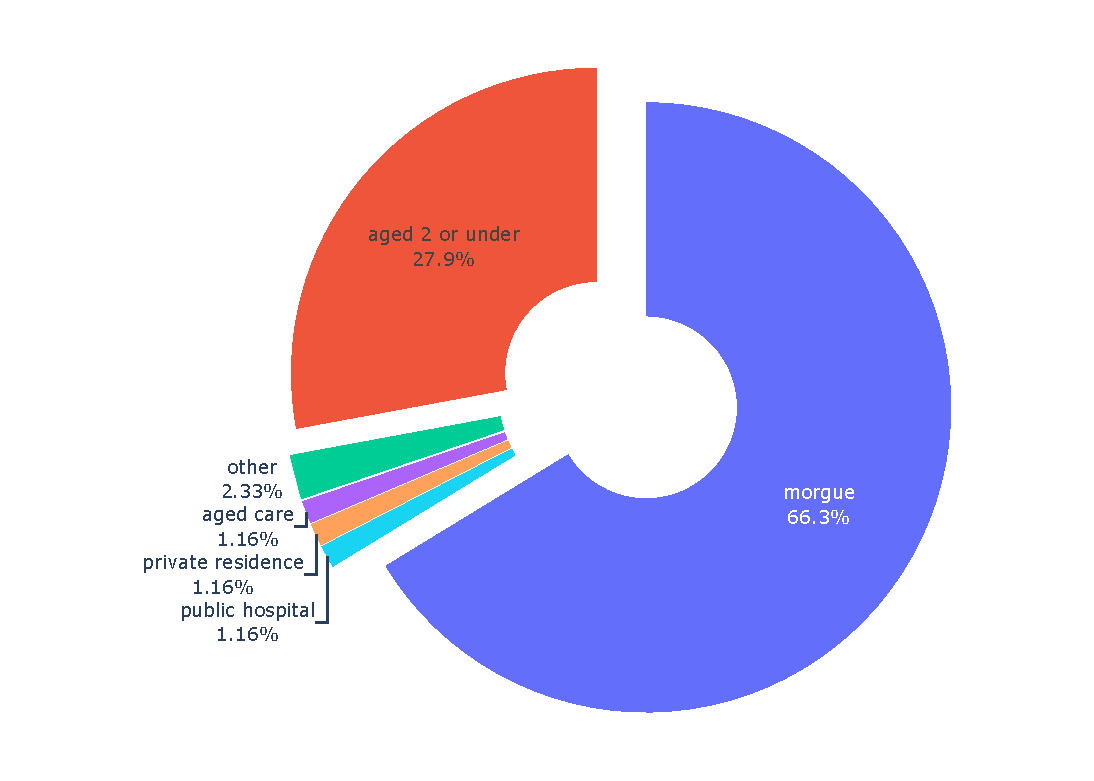
\includegraphics[width=0.9\textwidth]{REPORT/img/missing_suburbs.pdf}
\end{figure}

\paragraph{Merging with NSW geographical dataset}{When first exploring the geographical dataset, it was noted that there were 202 localities across New South Wales with the same name. This would present a significant issue when matching a suburb from the anatomy records to a suburb in the table. In order to deal with this, the Anatomy Registers dataset was first merged with the NSW Localities dataset using a \texttt{LEFT JOIN} in order to retain any duplicates. The dataset was then queried to extract any duplicated suburbs, outputting:
\begin{APAenumerate}
    \item Summer Hill (Inner West $\cdot$ Hunter Region)
    \item Punchbowl (Canterbury-Bankstown $\cdot$ Northern Rivers Region)
    \item Enmore (Inner West $\cdot$ New England Region)
    \item Darlington (Inner West $\cdot$ Hunter Region)
    \item Budgewoi
\end{APAenumerate}

After plotting the duplicates on a map, it was found that Summer Hill, Punchbowl, Enmore, and Darlington were all inner city suburbs having rural villages sharing their name. It was confirmed through corroborating their place of death entries that these patients were not sourced from their rural counterparts. Therefore, the duplicate entries closest to Sydney city were chosen to remain in the dataset.

Lastly, Budgewoi is a coastal town which is naturally divided into two by the Budgewoi Lake causing the duplicate suburb name. One Budgewoi geometry was chosen at random to remain in the dataset.
}

\subsection{Final dataset}

Ultimately, the work conducted in this section led to a cleaned, verified, and useable dataset containing 7510 entries (98.7\% of the original dataset) with nine original and three new attributes (see Table \ref{tab:full-schema}). The quality and utility of the Anatomy Registers dataset was significantly enhanced through employing data verification, validation, and transformation techniques. Furthermore, each step -- from ensuring data completeness to extracting geographical information -- was not only important in preparing the dataset for detailed analysis, but also served as a valuable case study in techniques that can be employed when handling archival data from other sources. 

\begin{table}[ht]
\centering
\caption{Schema of the Anatomy Registers dataset (* indicates a column not present in the original dataset)}
\label{tab:full-schema}
\begin{tabular}{llrl}
\toprule
\textbf{Attribute Name} & \textbf{Data Type} & \textbf{Missing} & \textbf{Description} \\
\midrule
id                      & Integer            & 0                      & Unique identifier for each entry \\
year                    & Integer            & 0                      & Year the body was received \\
age                     & Integer            & 0                      & Age at the time of death \\
death\_date             & Date               & 0                      & Date of the donor's death \\
reception\_date         & Date               & 1                      & Date body was received at the school \\
return\_date\_sepulture & Date               & 1645                   & Date body was returned for burial \\
burial\_date            & Date               & 4353                   & Date of the body's burial \\
death\_place            & String             & 0                      & Location of death \\
place\_code             & String             & 0                      & Coded place of death \\
death\_place\_category* & String             & 0                      & Categorised place of death \\
suburb*                 & String             & 0                      & Suburb extracted from death place \\
geometry*               & Geometry           & 0                      & Geospatial data for location \\
\bottomrule
\end{tabular}
\end{table}
\newpage
\section{Results and Discussion}

The initial phase of our project was dedicated to cleaning and validating the Anatomy Registers dataset. Given the large volume and arcane lettering of the handwritten records, the dataset was prone to numerous transcription errors. Our systematic approach, involving techniques such as regular expressions, was critical for enhancing the data's reliability and accuracy, making it suitable for further analysis. 

Following data validation, we focused on data transformation and feature extraction, particularly targeting the ``place of death'' attribute. This involved (a) categorising each entry by the type of institution the patient died in (e.g. private residence, public hospital etc.), and (b) extracting the suburb where the patient died in. This involved using text parsing and geographic information system (GIS) techniques, which facilitated the transition from basic descriptive statistics to a deeper geospatial analysis. The refinement of this data allowed us to generate comprehensive choropleth maps, illustrating the distribution and evolution of donor sources across NSW. 

The animated choropleth map (Figure \ref{fig:choropleth-comparison}), showing the most common category of death place per suburb through each decade from the 1880s to 1980s, revealed a notable shift in the sources of bodies for anatomical study. Prior to 1950, a majority of bodies originated from public and mental asylums, indicating a period when body donation was more stigmatised and the Medical School was heavily reliant on unclaimed bodies from such institutions for anatomical dissection. However, post-1960s, there was a significant increase in donors from private residences, indicating a shift in public perceptions towards body donation as a more accepted and personal choice. 

\begin{figure}[p]
    \centering
    \caption{A choropleth map showing the stark difference between the largely institution-reliant donor program in the 1950s and the influx of private donors in the 1960s.}
    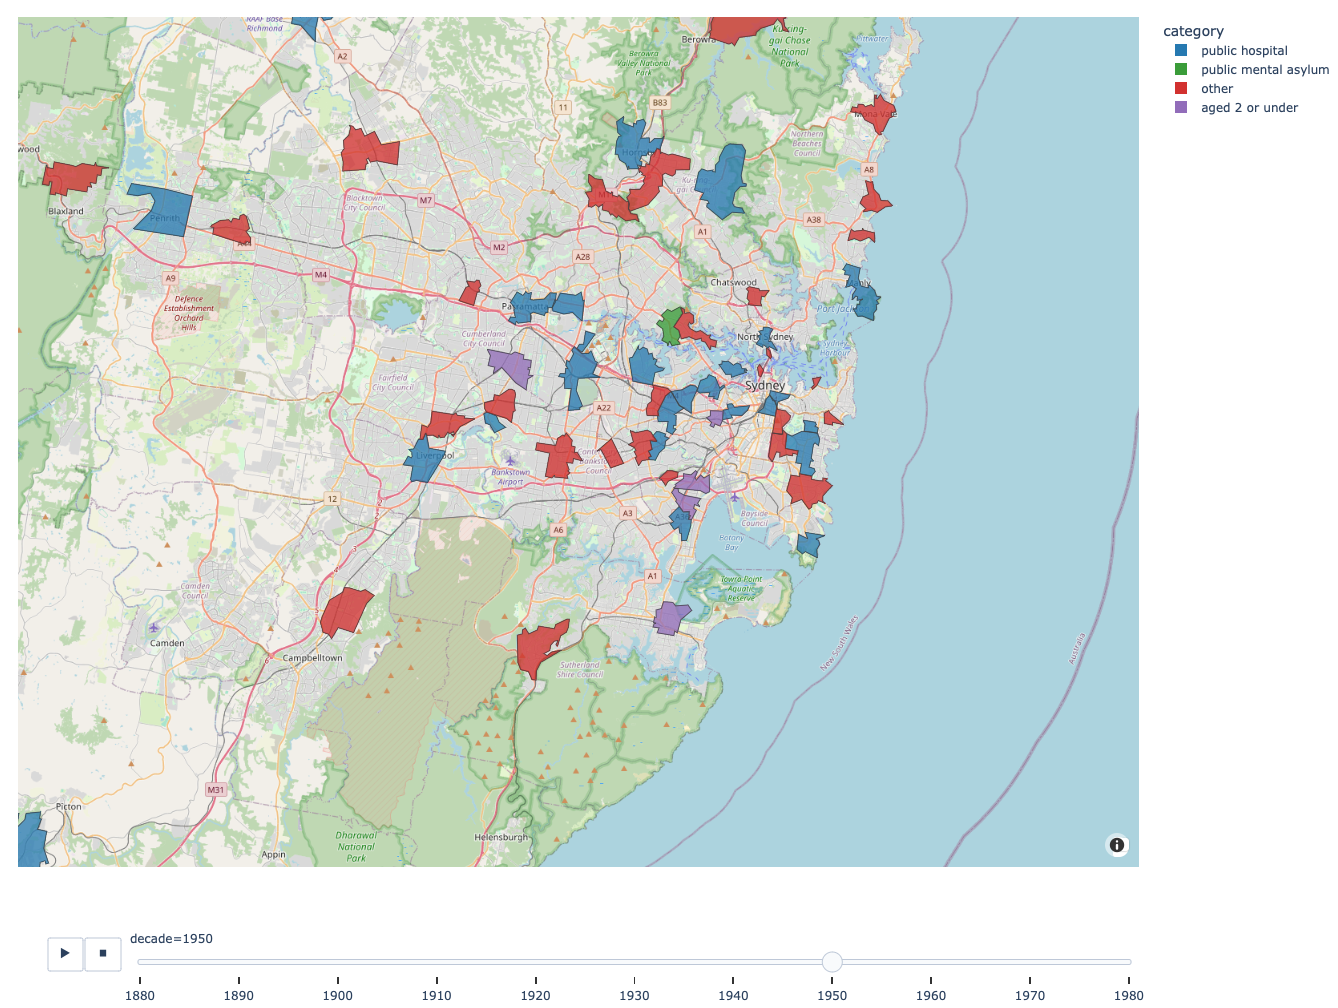
\includegraphics[width=0.95\textwidth]{REPORT/img/choropleth-1950.png}
    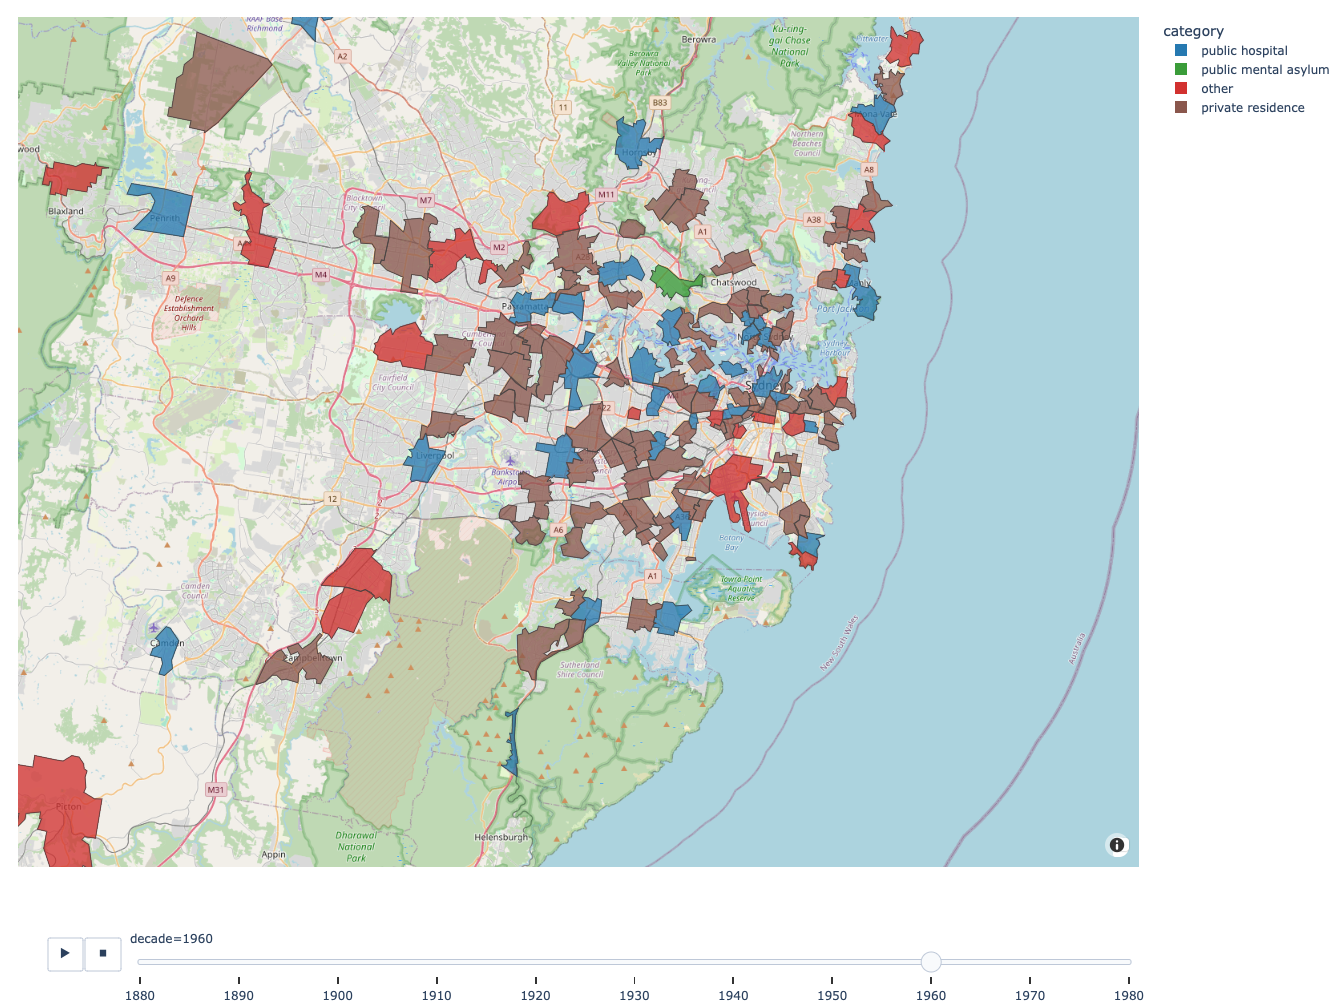
\includegraphics[width=0.95\textwidth]{REPORT/img/choropleth-1960.png}
    \label{fig:choropleth-comparison}
\end{figure}

This shift in attitude was coincident with the transition to a body donor program. Voluntary body donation steadily increased from the year 1916, when the first documented body donation was recorded, to the year 1960, where 118 out of 127 bodies admitted were registered or private donors, until ``by the late 1960s, a waiting list for would be donors had to be introduced, with restrictions on the registration of new donors sometimes lasting beyond a year'' \parencite{rebekah_jenkin}.

It appears that this trend of the public becoming more conscious over what happens to their body after they pass was not limited to just Australia. Indeed, Canada, the United Kingdom, and the United States also saw the upsurge of voluntary donation in the mid-20th century. In a similar study to the one conducted at the University of Sydney, anatomists at McGill University in Canada saw the first bequeathments (or ``gifts'' as they were originally called) of bodies in the 1950s and also witnessed the rate of donations increasing rapidly after the year 1965 \parencite{noel_2022_mcgill}. In the United Kingdom, it was in the late `40s that the newly-initiated National Health Service saw a ``dramatic'' change in public perceptions and saw the beginnings of bodies ``provided in a spirit of trust and generosity, by voluntary public donation'' \parencite{richardson_2006_ukdonors, jones_1991_nzdonors}. The United States also shared this trend despite limited ties to the UK and its legislature \parencite{garment_2007_usadonors}.\footnote{Canada and Australia's Anatomy Acts both aligned themselves closely to the original British Anatomy Act of 1832.} 

We cannot be certain for the reasons behind this uptrend in body donation during the 1950s and 1960s. This is because the way a society deals with death reflects the way its citizens live, and, as a result, any trends to due with bequeathment programs are a culmination of changes in society itself. 
\begin{quote}
A population boom, expansion of government, new legislation, changes in the population demographics, developments in science, and proliferation of mass media, all affected body acquisition. \parencite{garment_2007_usadonors}
\end{quote}
However, there are a few probable causes towards this trend.
\begin{enumerate}
    \item \textbf{The effects of World War II.} The widespread establishment of blood transfusion services during World War II had a profound influence on public willingness to contribute to medical science, not just through blood donation but also through body donation for dissection. As \citeauthor{richardson_2006_ukdonors} notes, the collective effort in wartime medical services likely fostered a sense of communal responsibility towards advancing medical knowledge and healthcare, which persisted into the post-war era \parencite{richardson_2006_ukdonors}. This shift contributed to a greater acceptance of body donation as another form of contribution to the medical field.
    \item \textbf{Shifts in religious beliefs.} The mid-20th century witnessed significant shifts in societal and religious attitudes towards the human body post-mortem. As traditional views on the spiritual significance of the corpse began to wane, alongside an increase in the popularity of cremation, public attitudes towards scientific medicine and body donation started to change. \citeauthor{jones_1991_nzdonors} touch on how these evolving beliefs, coupled with an enhanced understanding of the medical benefits of body donation, led to broader acceptance and support of anatomical donations \parencite{jones_1991_nzdonors}.
    \item \textbf{The cost of dying.} The American funeral industry boomed due to the popularisation of embalming in the mid-19th century, and alongside this, the price of funerals skyrocketed. According to \citeauthor{garment_2007_usadonors}, three pieces of journalism were instrumental in bringing to light the excessive costs paid to die in the country: ``The High Cost of Dying'' by Bill Davidson, ``Can You Afford to Die'' by Roul Tunley, and ``The American Way of Death'' by Jessica Mitford, all published in the `50s and `60s. Mitford's book contained the first publicly available list of schools that would accept bodies for donation, provided as an alternative to succumbing to exorbitant funeral costs. It is likely that Davidson, Tunley, and Mitford's works helped increase the public's awareness of alternatives, a key one being body donor programs.
\end{enumerate}


These insights into historical and societal trends are crucial as they highlight the impact of digitising and analysing historical datasets, echoing the broader themes discussed in our literature review. Just as the analysis of ship logbooks \parencite{petrakis_2021_ship} provided a window into the psychological landscape of historical maritime transitions, our project shows the evolution of societal attitudes towards a once-stigmatised aspect in medical science.

\subsection{Limitations}
Despite our achievements, the project faced certain limitations, particularly in the categorisation of the `place of death' entries. A significant number of entries remained classified under ``Other'', including those with misspelled addresses and ambiguous locations, indicating the complexity of interpreting such historical data accurately. This limitation underscores the need for more advanced natural language processing techniques and machine learning models to handle the intricacies of data entry. Additionally, manual review and enhancement of the categorisation process would likely improve data accuracy and the quality of insights derived from our analysis.
\newpage
\section{Conclusion}

The exploration of the Anatomy Registers from The University of Sydney Medical School has proven both challenging and enlightening. This project illuminated changes in historical practices and societal attitudes towards body donation, while reinforcing the value of digitising and analyzing historical datasets.

Working with manually transcribed data introduces significant complexities, primarily due to the extensive data cleaning and validation required to ensure analysis reliability. Transforming the "place of death" data into a structured format enabled us to identify geographical patterns and temporal changes in body donation sources. Our geospatial analyses, particularly the animated choropleth map, visually narrated the evolution of societal norms from a reliance on unclaimed bodies from public institutions to an increase in donations from private residences, highlighting a significant shift in public perception towards body donation.

Nevertheless, the project encountered some limitations, especially in data categorisation. The large number of entries labeled as "Other" highlights the potential for enhancements in methodology through employing advanced technologies like machine learning and natural language processing.

Future endeavors will likely focus on further refining data standardization processes and exploring our initial research questions, such as using the cause of death attribute to trace the emergence of new medical fields like psychiatry through dynamic topic modeling. This could potentially reveal historical trends in medical terminology and diagnostics.

In conclusion, while this project has provided valuable insights and advanced the field of digital humanities in relation to anatomical history, it also underscores the continuous need for innovation and reflection in the methodologies we employ to examine our past so that we may learn from it.


%%%%%%% BIBLIOGRAPHY %%%%%%%%%

\nocite{*} % Add all entries from bibliography file
% %\addcontentsline{toc}{section}{References}
\printbibliography

%%%%%%% APPENDICES %%%%%%%%%

\appendix

\section{}

All the code used to clean and analyse the Anatomy Registers dataset can be found at \url{https://github.com/antrikshdhand/SCDL3991-research}.

\end{document}